% ============================================================================
%  李雅普诺夫稳定性定理及其控制应用
%  编译：latexmk -xelatex lyapunov-stability.tex
%  作者：刘昊岳
% ============================================================================
\PassOptionsToPackage{table}{xcolor}
\documentclass[11pt, a4paper, UTF8, fontset=none]{ctexart}

% --------------------------------- 版面 ---------------------------------
\usepackage[a4paper, margin=2.2cm, headheight=15pt, headsep=8pt]{geometry}
\linespread{1.13}

% --------------------------------- 字体 ---------------------------------
\usepackage{fontspec}
\usepackage{unicode-math}
\setmainfont{TeX Gyre Pagella}
\setsansfont{TeX Gyre Heros}
\setmonofont{Latin Modern Mono}[Scale=0.92]
\setmathfont{TeX Gyre Pagella Math}
\setCJKmainfont{Noto Serif CJK SC}[AutoFakeSlant=0.15]
\setCJKsansfont{Noto Sans CJK SC}[AutoFakeSlant=0.15]
\setCJKmonofont{Noto Sans Mono CJK SC}

% --------------------------------- 宏包 ---------------------------------
\usepackage{graphicx}
\usepackage{amsmath}
\usepackage{amsthm}
\usepackage{booktabs, array, tabularx}
\usepackage{enumitem}
\usepackage{xcolor}
\usepackage[most]{tcolorbox}
\usepackage{titlesec}
\usepackage{fancyhdr}
\usepackage{caption}
\usepackage{float}
\usepackage[colorlinks=true, linkcolor=navy, urlcolor=teal, citecolor=navy]{hyperref}

% --------------------------------- 色彩 ---------------------------------
\definecolor{navy}{HTML}{1E3A8A}
\definecolor{teal}{HTML}{0F766E}
\definecolor{amber}{HTML}{B45309}
\definecolor{redalert}{HTML}{991B1B}
\definecolor{muted}{HTML}{5B6673}
\definecolor{rulecolor}{HTML}{D5DEE9}
\definecolor{softblue}{HTML}{EFF6FF}
\definecolor{softteal}{HTML}{F0FDFA}
\definecolor{softamber}{HTML}{FFFBEB}

% ------------------------------- 超链接 ---------------------------------
\hypersetup{
    pdftitle={李雅普诺夫稳定性定理及其控制应用},
    pdfauthor={刘昊岳},
    pdfsubject={非线性控制、稳定性理论与 Lyapunov 方法},
    pdfkeywords={李雅普诺夫函数, 稳定性, CLF, LQR, Sontag 公式, 反步法}
}

% ------------------------------- 列表间距 -------------------------------
\setlist[itemize]{label=\textbullet, topsep=3pt, itemsep=2pt, leftmargin=1.4em}
\setlist[enumerate]{topsep=3pt, itemsep=2pt, leftmargin=1.8em}

% ------------------------------- 页眉页脚 -------------------------------
\pagestyle{fancy}
\fancyhf{}
\fancyhead[L]{\small\sffamily\color{muted}李雅普诺夫稳定性定理及其控制应用}
\fancyhead[R]{\small\sffamily\color{muted}作者：刘昊岳}
\fancyfoot[C]{\small\sffamily\color{muted}\thepage}
\renewcommand{\headrulewidth}{0.4pt}
\renewcommand{\footrulewidth}{0pt}

% ------------------------------- 标题样式 -------------------------------
\titleformat{\section}{\Large\bfseries\sffamily\color{navy}}{\thesection}{0.7em}{}[{\color{rulecolor}\titlerule}]
\titleformat{\subsection}{\large\bfseries\sffamily\color{navy!85!black}}{\thesubsection}{0.6em}{}
\titleformat{\subsubsection}{\normalsize\bfseries\sffamily\color{teal!90!black}}{\thesubsubsection}{0.5em}{}
\titlespacing*{\section}{0pt}{18pt}{10pt}
\titlespacing*{\subsection}{0pt}{14pt}{7pt}

% ------------------------------- 题注样式 -------------------------------
\DeclareCaptionLabelFormat{cn}{\textbf{\sffamily\color{navy}#1~#2：}}
\captionsetup{labelformat=cn, labelsep=none, font=small, justification=centering, skip=6pt}
\captionsetup[table]{position=top, skip=5pt}
\captionsetup[figure]{position=bottom}

% ------------------------------- 定理样式 -------------------------------
\newtheoremstyle{cnthm}
  {8pt}{8pt}
  {\normalfont}
  {0pt}
  {\bfseries\sffamily\color{navy}}
  {}
  {0.5em}
  {\thmname{#1}\thmnumber{ #2}\thmnote{\ （#3）}：}
\theoremstyle{cnthm}
\newtheorem{theorem}{定理}[section]
\newtheorem{lemma}[theorem]{引理}
\newtheorem{proposition}[theorem]{命题}
\newtheorem{corollary}{推论}[section]
\newtheorem{definition}{定义}[section]
\newtheorem{remark}{注}[section]
\newtheorem{example}{例}[section]
\renewcommand{\proofname}{证明}
\renewcommand{\qedsymbol}{$\rule[0.12ex]{0.7ex}{0.7ex}$}

% ------------------------------- 提示框 ---------------------------------
\newtcolorbox{keybox}[1][核心结论]{
  enhanced, breakable, colback=softblue, colframe=navy!65,
  boxrule=0pt, leftrule=2.5pt, arc=2pt, left=9pt, right=9pt, top=8pt, bottom=8pt,
  title={#1}, fonttitle=\bfseries\sffamily\small, coltitle=white, colbacktitle=navy,
  before skip=9pt, after skip=9pt
}
\newtcolorbox{warnbox}[1][注意]{
  enhanced, breakable, colback=softamber, colframe=amber!70,
  boxrule=0pt, leftrule=2.5pt, arc=2pt, left=9pt, right=9pt, top=8pt, bottom=8pt,
  title={#1}, fonttitle=\bfseries\sffamily\small, coltitle=white, colbacktitle=amber,
  before skip=9pt, after skip=9pt
}

% ------------------------------- 数学记号 -------------------------------
\newcommand{\R}{\mathbb{R}}
\newcommand{\X}{\mathcal{X}}
\newcommand{\U}{\mathcal{U}}
\newcommand{\Y}{\mathcal{Y}}
\newcommand{\T}{\mathcal{T}}
\newcommand{\norm}[1]{\lVert #1\rVert}
\newcommand{\abs}[1]{\lvert #1\rvert}
\newcommand{\Lf}{L_f}
\newcommand{\Lg}{L_g}
\DeclareMathOperator{\dist}{dist}
\DeclareMathOperator*{\argmin}{arg\,min}

% ------------------------------- 段落与表格 -----------------------------
\setlength{\parindent}{0pt}
\setlength{\parskip}{6pt}
\setlength{\emergencystretch}{1.5em}
\renewcommand{\arraystretch}{1.28}

\title{\textbf{\LARGE 李雅普诺夫稳定性定理及其控制应用}\\[8pt]
\large 从“不解方程判稳”到“构造控制律”}
\author{作者：刘昊岳}
\date{2026年10月}

\begin{document}

\maketitle

\begin{abstract}
\noindent 本文从状态空间系统的公理化描述出发，给出李雅普诺夫稳定、渐近稳定与全局渐近稳定三个定理的完整陈述与证明。定理~1 的证明围绕球面 $\norm{x}=r$ 上 $V$ 的最小值 $m$、初值足够近使 $V(x(0))<m$、以及 $\dot V\le 0$ 保证轨迹碰不到该球面这一逻辑展开；定理~2、3 在此基础上加入收敛性论证，并说明径向无界条件如何把局部结论提升为全局结论。随后讨论线性系统的 Lyapunov 方程、LQR 与 Riccati 方程的关系，以及控制李雅普诺夫函数（CLF）、Sontag 公式、反步法、滑模控制与自适应控制中的 Lyapunov 思想。最后用一个二阶非线性系统的闭环设计，展示“给定 $V$、选择 $u$ 使 $\dot V<0$”的完整流程，并指出该方法的适用范围与局限。
\end{abstract}

\tableofcontents


% ============================================================================
\section{引言：李雅普诺夫方法解决什么问题}
% ============================================================================

稳定性讨论的不是某一条事先算好的轨迹，而是\emph{所有从平衡点附近出发的解}在初值小扰动下是否始终留在平衡点附近。对线性系统 $\dot x=Ax$，这可以化归为特征值实部的符号；但对一般的非线性系统
\begin{equation}
  \dot x=f(x),\qquad f(0)=0,
  \label{eq:autonomous}
\end{equation}
显式求解往往既不可能，也没有必要。李雅普诺夫第二方法（直接法）的核心思想是：不去解方程，而是找一个标量函数 $V(x)$，它像“能量”一样在平衡点取最小值，并沿轨迹不增；只要这样的 $V$ 存在，就能在不求解的前提下断定稳定性。

李雅普诺夫方法通常从自治系统 \eqref{eq:autonomous} 讲起：$x\in\R^n$ 是状态，$f$ 是状态演化函数，$0$ 是平衡点。把输入 $u$ 显式写出来后，系统变为 $\dot x=f(x,u,t)$；当 $u$ 由状态反馈 $u=\kappa(x,t)$ 给定时，闭环又回到一个（可能非自治的）状态方程。因此，开环系统上的稳定性语言可以自然迁移到闭环系统：$V$ 沿着“系统 + 控制器”的联合轨迹求导，稳定性就变成对 $\dot V$ 的符号检查。

同一个 $V$ 可以朝两个方向使用。\textbf{分析}是“给定 $f$，寻找 $V$”，找到一个合适的 $V$ 就证明了稳定性；\textbf{设计}是“给定 $V$，选择 $u$ 使 $\dot V<0$”，把稳定性要求反过来当作控制律的约束。控制李雅普诺夫函数、Sontag 公式、LQR、反步法、滑模与自适应控制，本质上都是这一对偶的不同实现。理解这条主线，比记住一堆彼此孤立的判据更重要。

本文结构如下：第~\ref{sec:prelim} 节给出状态空间系统的公理化描述、术语表与稳定性定义；第~\ref{sec:theorems} 节完整陈述并证明三个稳定性定理，并简介 LaSalle 不变集原理；第~\ref{sec:linear} 节讨论线性系统与 Lyapunov 方程；第~\ref{sec:design} 节说明如何用 Lyapunov 方法指导控制设计；第~\ref{sec:example} 节给出一个闭环设计例子；第~\ref{sec:scope} 节讨论适用范围、局限与总结。

% ============================================================================
\section{预备：系统、平衡点与 Lyapunov 函数}
\label{sec:prelim}
% ============================================================================

\subsection{术语与符号}

表~\ref{tab:notation} 汇总了本文反复使用的记号。需要强调：$x,u,y$ 都是向量（标量是 $m=p=1$ 的特例），而 $V$ 始终是\textbf{标量函数}；$\dot V$ 是 $V$ 沿轨迹的\textbf{标量方向导数}，不是矩阵，也不是把 $\dot x$ 写成矩阵后的某种范数。

\begin{table}[H]
\centering
\small
\begin{tabularx}{\textwidth}{@{}>{\raggedright\arraybackslash}p{2.55cm}>{\raggedright\arraybackslash}p{3.25cm}X@{}}
\toprule
符号 & 名称（中/英） & 含义与所属空间 \\
\midrule
$x\in\R^n$ & 状态（state） & 系统内部构型；$x(t)\in\X\subseteq\R^n$，$n$ 为状态维数。 \\
$u\in\R^m$ & 输入、控制（input, control） & 外部施加的作用；$u(t)\in\U\subseteq(\R^m)^{\T}$，$m$ 为输入维数。 \\
$y\in\R^p$ & 输出（output） & 可测量或关心的量；$y(t)\in\Y\subseteq\R^p$，$p$ 为输出维数。 \\
$f$ & 状态演化函数 & $\dot x=f(x,u,t)$，决定状态空间的向量场。 \\
$h$ & 输出映射 & $y=h(x,u,t)$。 \\
$V(x)$ & 李雅普诺夫函数（Lyapunov function） & 正定标量函数，$V:\X\to\R_{\ge0}$，$V(0)=0$；候选的“能量”。 \\
$\dot V(x)$ & 沿轨迹方向导数 & $\dot V(x)=\nabla V(x)^\top f(x,u)$，标量；不是矩阵，也不是 $\dot x$ 的矩阵范数。 \\
$V(x)=c$ & 李雅普诺夫面/等值面（level set） & 使 $V$ 取常值 $c$ 的曲面；局部情形下 $c>0$ 的等值面围住原点。 \\
\bottomrule
\end{tabularx}
\caption{术语与符号。状态、输入、输出都是向量；$V$ 与 $\dot V$ 都是标量。}
\label{tab:notation}
\end{table}

\textbf{SISO 与 MIMO 的区别。}当 $m=p=1$ 时系统是单输入单输出（SISO），$u(t),y(t)$ 都是标量，控制方向可以直接由 $\Lg V$ 的符号判断：$\Lg V>0$ 时增大 $u$ 会使 $V$ 增大，$\Lg V<0$ 时相反。当 $m,p>1$ 时是多输入多输出（MIMO），$u$ 与 $y$ 都是向量，$\Lg V=\nabla V^\top g$ 是一个 $1\times m$ 的行向量，它给出 $V$ 对各个输入通道的敏感度；此时“往哪个方向打控制”本身就是一个需要选择的问题。CLF 的不等式 $\dot V<0$ 仍然是标量不等式，与 $m$ 无关，但输入方向、执行器饱和、通道耦合与权重矩阵 $R$ 都会影响控制的可行性。LQR 中的 $R\in\R^{m\times m}$ 与 Sontag 公式中的 $\norm{\Lg V}$ 正是 MIMO 情形的直接体现。

\subsection{状态空间系统的公理化描述}

一个连续时间状态空间系统由以下对象构成：
\begin{itemize}
  \item 时间集 $\T=\R$；
  \item 输入空间 $\U\subseteq(\R^m)^{\T}$，其元素是定义在时间轴上的输入信号 $u(\cdot)$；
  \item 状态空间 $\X\subseteq\R^n$；
  \item 输出空间 $\Y\subseteq\R^p$；
  \item 状态演化映射
  \begin{equation}
    \varphi:\T\times\T\times\X\times\U\longrightarrow\X,
    \qquad (t,t_0,x_0,u)\longmapsto \varphi(t,t_0,x_0,u),
  \end{equation}
  它给出从 $t_0$ 时刻状态 $x_0$ 出发、在输入 $u$ 作用下于 $t$ 时刻到达的状态。
\end{itemize}
映射 $\varphi$ 满足三条公理：
\begin{enumerate}[label=(A\arabic*)]
  \item \textbf{恒等性}：$\varphi(t,t,x_0,u)=x_0$；
  \item \textbf{因果性}：若 $u|_{[t_0,t)}=u'|_{[t_0,t)}$，则 $\varphi(t,t_0,x_0,u)=\varphi(t,t_0,x_0,u')$；
  \item \textbf{拼接性}：$\varphi(t_2,t_0,x_0,u)=\varphi\bigl(t_2,t_1,\varphi(t_1,t_0,x_0,u),u\bigr)$。
\end{enumerate}
因果性说明“未来不影响现在”，拼接性说明“从 $t_0$ 到 $t_2$ 的演化可以拆成 $t_0\to t_1$ 与 $t_1\to t_2$ 两段。工程上通常把上述公理系统写成微分方程
\begin{equation}
  \dot x=f(x,u,t),\qquad y=h(x,u,t),
  \label{eq:state-space}
\end{equation}
其中 $f$ 与 $h$ 足够光滑，使得初值问题存在唯一解。此时 $\varphi(t,t_0,x_0,u)$ 就是解 $x(t)$，输出为 $y(t)=h(x(t),u(t),t)$。线性时不变（LTI）形式是
\begin{equation}
  \dot x=Ax+Bu,\qquad y=Cx+Du,
  \label{eq:lti}
\end{equation}
其中 $A\in\R^{n\times n}$、$B\in\R^{n\times m}$、$C\in\R^{p\times n}$、$D\in\R^{p\times m}$，$x\in\R^n$、$u\in\R^m$、$y\in\R^p$。

图~\ref{fig:system} 给出状态空间系统的框图：左侧输入 $u(t)$ 进入系统 $\Sigma$，右侧输出 $y(t)$，内部状态 $x(t)$ 用虚线引出。图~\ref{fig:structure} 给出对应的状态变量图：每一路积分器把 $\dot x_i$ 变成 $x_i$，加法器与比例器实现 $f_i$ 与 $h$，输入 $u$ 进入加法器，输出 $y$ 由状态与输入共同决定。

\begin{figure}[H]
\centering
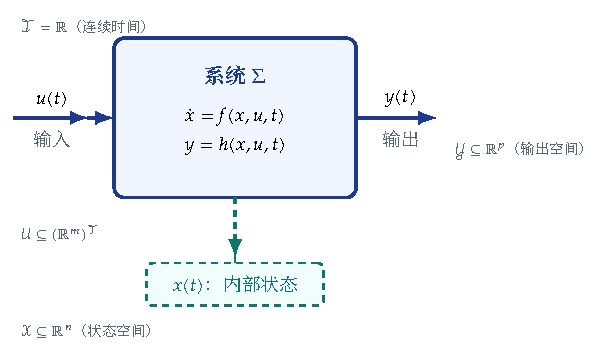
\includegraphics[width=0.92\textwidth]{figures/fig1-system.pdf}
\caption{状态空间系统框图。读图要点：$u(t)$ 是外部输入，$y(t)$ 是输出，二者都属于外部信号；$x(t)$ 是系统内部状态，通常不能直接测量，只能通过输出或状态估计获得。图中的 $\dot x=f(x,u,t)$ 与 $y=h(x,u,t)$ 分别是状态演化律与输出映射。}
\label{fig:system}
\end{figure}

\begin{figure}[H]
\centering
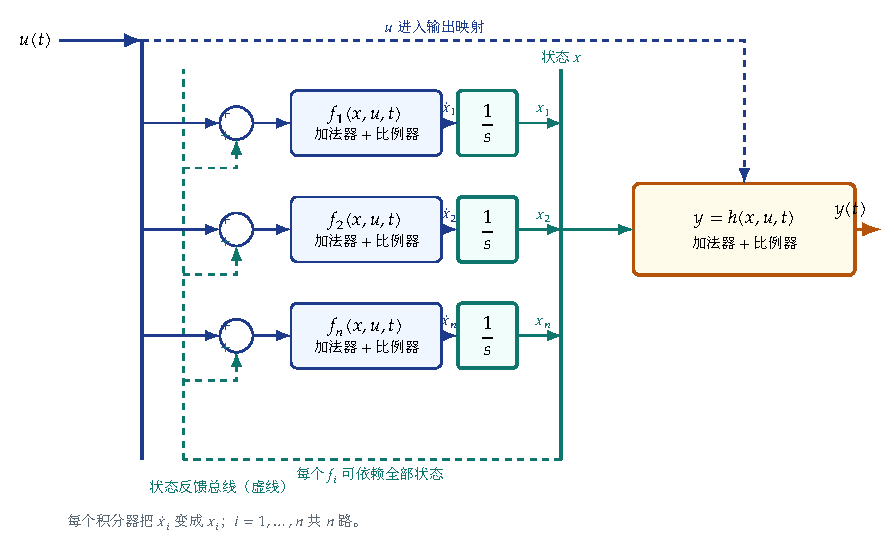
\includegraphics[width=\textwidth]{figures/fig2-structure.pdf}
\caption{状态变量图（模拟结构图）。读图要点：每个积分器以 $\dot x_i$ 为输入、以 $x_i$ 为输出，箭头方向不能反；所有状态经状态总线反馈到各 $f_i$ 的加法器，输入 $u$ 也进入加法器；输出映射 $h$ 同时接收状态与输入，产生 $y(t)$。图中省略了各通道的具体增益，只保留结构。}
\label{fig:structure}
\end{figure}

\subsection{平衡点、稳定性、吸引性与吸引域}

不失一般性，本文讨论原点 $x^\ast=0$ 处的稳定性。若平衡点 $x^\ast\ne0$，令 $z=x-x^\ast$ 即可平移回原点。对自治系统 \eqref{eq:autonomous}，$0$ 是平衡点意味着 $f(0)=0$；对带输入的系统，通常考虑零输入平衡点 $f(0,0,t)=0$，或考虑闭环系统。

\begin{definition}[李雅普诺夫稳定]
平衡点 $0$ 是（李雅普诺夫）稳定的，如果对任意 $\varepsilon>0$，存在 $\delta=\delta(\varepsilon,t_0)>0$，使得只要 $\norm{x_0}<\delta$，就有
\begin{equation}
  \norm{x(t;t_0,x_0)}<\varepsilon,\qquad \forall\,t\ge t_0.
  \label{eq:stable}
\end{equation}
若 $\delta$ 可取为与 $t_0$ 无关，则称一致稳定。
\end{definition}

\begin{definition}[吸引与渐近稳定]
平衡点 $0$ 是吸引的，如果存在 $\delta_0>0$，使得 $\norm{x_0}<\delta_0$ 蕴含
\begin{equation}
  \lim_{t\to\infty}x(t;t_0,x_0)=0.
\end{equation}
若 $0$ 既稳定又吸引，则称它是渐近稳定的。若 $\delta_0$ 可取为任意大（即所有初值都收敛），则称全局渐近稳定。
\end{definition}

\begin{definition}[吸引域]
使 $\lim_{t\to\infty}x(t;t_0,x_0)=0$ 的所有初值 $x_0$ 的集合称为 $0$ 的吸引域（domain of attraction），记为 $\mathcal{D}$。
\end{definition}

这里要特别澄清一个常见误解：稳定性不是“某一条轨迹有界”，而是“\textbf{从原点附近任意初值出发的所有解}都不逃离原点附近”。图~\ref{fig:level} 给出几何直觉：$V=c$ 的等值线像一圈圈“围栏”，$\dot V\le0$ 保证轨迹只能向 $V$ 更小的内层走，而不能穿到外层去。

\begin{remark}
稳定但不吸引的例子是无阻尼谐振子 $\ddot x+\omega^2x=0$：相平面上的轨迹是闭合椭圆，初值小扰动不会发散，但也不会收敛到原点。吸引但不稳定的例子在一般非线性系统中存在（某些解会被“拉向”原点，但另一些任意接近原点的解会先逃出任意大的范围），因此“吸引”不能替代“稳定”。渐近稳定按定义同时包含二者。
\end{remark}

\subsection{正定函数、径向无界性与沿轨迹导数}

\begin{definition}[正定、半正定与负定]
设 $D\subseteq\R^n$ 是包含原点的区域。函数 $V:D\to\R$ 称为在 $D$ 上正定，如果 $V(0)=0$ 且对任意 $x\in D\backslash\{0\}$ 有 $V(x)>0$。若 $-V$ 正定，则称 $V$ 负定；若 $V(x)\ge0$ 对一切 $x\in D$ 成立，则称半正定。若 $V:\R^n\to\R$ 正定且满足
\begin{equation}
  \norm{x}\to\infty\quad\Longrightarrow\quad V(x)\to\infty,
  \label{eq:radial}
\end{equation}
则称 $V$ 径向无界（radially unbounded，或称 proper）。
\end{definition}

\begin{definition}[沿轨迹的方向导数]
设 $V$ 连续可微，系统为 \eqref{eq:state-space}。$V$ 沿轨迹的导数为
\begin{equation}
  \dot V(x)=\nabla V(x)^\top f(x,u)
  =\sum_{i=1}^{n}\frac{\partial V}{\partial x_i}(x)\,f_i(x,u).
  \label{eq:dotV}
\end{equation}
\end{definition}

\begin{warnbox}[$\dot V$ 是标量，不是矩阵]
式~\eqref{eq:dotV} 中 $\nabla V(x)$ 是 $n\times1$ 的列向量，$f(x,u)$ 也是 $n\times1$ 的列向量，$\nabla V^\top f$ 是 $1\times1$ 的标量。它表示“沿向量场方向 $V$ 的变化率”，不是 Jacobian 矩阵，也不是 $\dot x$ 的某种矩阵范数。很多记号混乱都源于把 $\dot V$ 误写成矩阵乘积；只要记住“行向量乘列向量得到一个数”，就不会出错。
\end{warnbox}

几何上，$V(x)=c$ 是 $V$ 的等值面（李雅普诺夫面）。若 $\dot V(x)\le0$，则沿轨迹 $V(x(t))$ 单调不增，轨迹只能停留在同一等值面上或进入 $V$ 更小的等值面；若 $\dot V(x)<0$，则严格进入更小的等值面。图~\ref{fig:level} 左图用同心闭合曲线展示了这一点，右图把 $V$ 想象成一个“能量碗”，轨迹像小球沿碗壁下滑。

\begin{figure}[H]
\centering
\begin{minipage}[b]{0.56\textwidth}
\centering
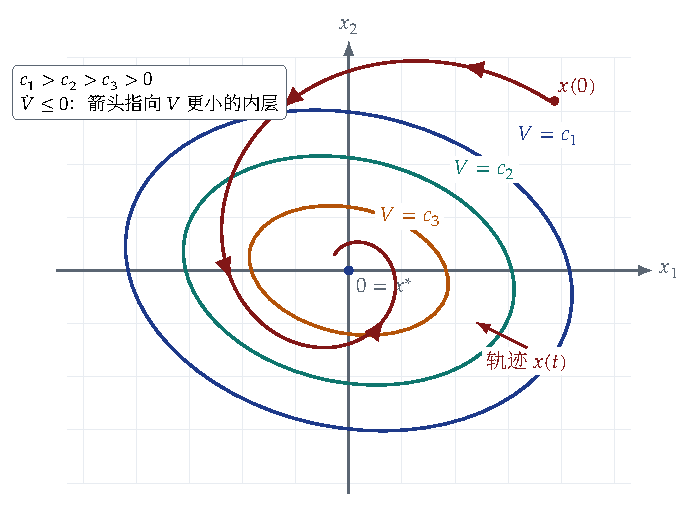
\includegraphics[width=\linewidth]{figures/fig3-level-sets.pdf}\\[-1pt]
{\small (a) 等值线与轨迹（严格示意）}
\end{minipage}\hfill
\begin{minipage}[b]{0.40\textwidth}
\centering
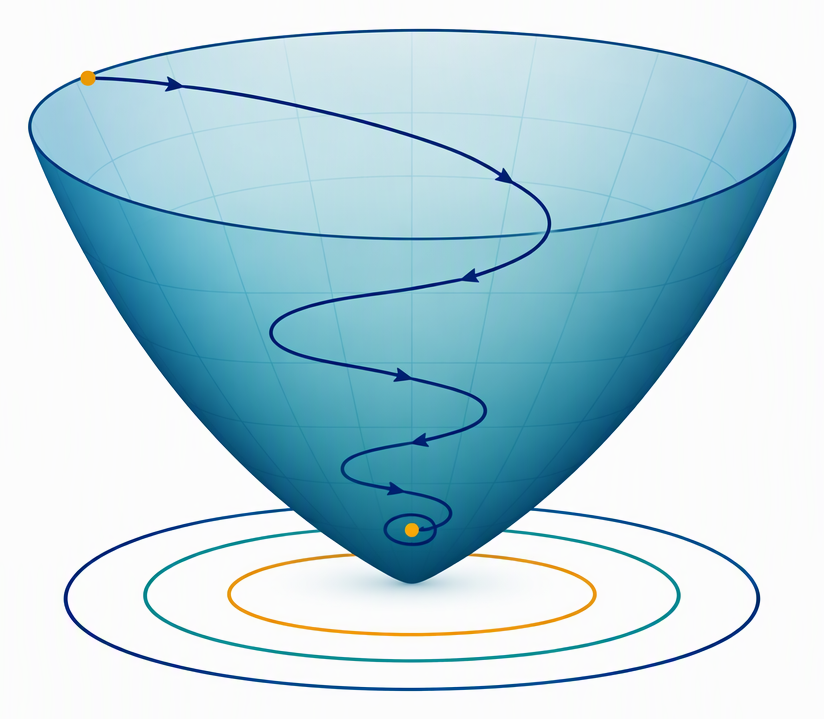
\includegraphics[width=\linewidth]{figures/fig3-energy-bowl.png}\\[-1pt]
{\small (b) 能量碗直观图（生图示意）}
\end{minipage}
\caption{李雅普诺夫等值线与轨迹。读图要点：左图中 $c_1>c_2>c_3>0$，三条闭合曲线是 $V=c_1,c_2,c_3$；红色轨迹从外层穿过等值线进入内层，所有箭头都指向 $V$ 更小的方向，绝不能画反。右图把 $V$ 看作能量碗，轨迹向碗底（原点）滑落，仅用于建立直觉；严格的等值线与方向以左图为准。}
\label{fig:level}
\end{figure}

最后引入一个在非自治系统与定量估计中常用的记号。连续函数 $\alpha:[0,a)\to[0,\infty)$ 称为 $\mathcal{K}$ 类函数，如果它严格递增且 $\alpha(0)=0$。若 $V$ 正定，则存在 $\mathcal{K}$ 类函数 $\alpha_1,\alpha_2$ 使得
\begin{equation}
  \alpha_1(\norm{x})\le V(x)\le\alpha_2(\norm{x})
  \label{eq:classK}
\end{equation}
在局部成立；若 $V$ 径向无界，则 $\alpha_1$ 可取为定义在 $[0,\infty)$ 上的 $\mathcal{K}_\infty$ 类函数。式~\eqref{eq:classK} 把“$V$ 正定”翻译成“$V$ 被 $\norm{x}$ 从两侧夹住”，在证明收敛速度时很有用。

% ============================================================================
\section{三个稳定性定理及证明}
\label{sec:theorems}
% ============================================================================

本节始终假设 $0$ 是系统 \eqref{eq:autonomous} 的平衡点，$f$ 在包含原点的区域 $D$ 上局部 Lipschitz，$V:D\to\R$ 连续可微。三个定理的差别只在于对 $V$ 与 $\dot V$ 的条件逐级加强：定理~\ref{thm:stable} 只要 $\dot V\le0$，定理~\ref{thm:asym} 要求 $\dot V$ 负定，定理~\ref{thm:global} 再要求 $V$ 径向无界。证明的主线也逐级递进：先证“碰不到球面”，再证“$V$ 的极限只能为 $0$”，最后用径向无界把局部紧性换成全局紧性。

\subsection{定理 1：李雅普诺夫稳定}

\begin{theorem}[李雅普诺夫稳定定理]
\label{thm:stable}
设 $D\subseteq\R^n$ 是包含原点的开区域，$f:D\to\R^n$ 局部 Lipschitz 且 $f(0)=0$。若存在连续可微函数 $V:D\to\R$ 满足
\begin{enumerate}[label=(\roman*)]
  \item $V(0)=0$，且对任意 $x\in D\backslash\{0\}$ 有 $V(x)>0$（正定）；
  \item 沿系统 \eqref{eq:autonomous} 的方向导数满足
  \begin{equation}
    \dot V(x)=\nabla V(x)^\top f(x)\le0,\qquad \forall\,x\in D,
    \label{eq:stable-condition}
  \end{equation}
\end{enumerate}
则平衡点 $0$ 是李雅普诺夫稳定的。
\end{theorem}

\begin{proof}
给定任意 $\varepsilon>0$。取 $r\in(0,\varepsilon]$ 足够小，使得闭球 $\bar B_r=\{x:\norm{x}\le r\}$ 包含在 $D$ 内。球面
\begin{equation}
  S_r=\{x\in\R^n:\norm{x}=r\}
\end{equation}
是紧集，$V$ 在 $S_r$ 上连续且处处为正，因此最小值
\begin{equation}
  m=\min_{x\in S_r}V(x)>0
  \label{eq:sphere-min}
\end{equation}
存在且严格为正。这是整个证明的支点：\textbf{球面上的 $V$ 有一个正的下界 $m$}。

由于 $V(0)=0$ 且 $V$ 在 $0$ 处连续，存在 $\delta\in(0,r)$，使得
\begin{equation}
  \norm{x}<\delta\quad\Longrightarrow\quad V(x)<m.
  \label{eq:delta-V}
\end{equation}

现在取任意初值 $x_0\in B_\delta$，设 $x(t)=x(t;0,x_0)$ 是其最大解。反设存在某个 $t_1>0$ 使 $\norm{x(t_1)}\ge r$。由解对时间的连续性，集合
\begin{equation}
  \{t\ge0:\norm{x(t)}=r\}
\end{equation}
非空，令 $t^\ast=\inf\{t\ge0:\norm{x(t)}=r\}$。则在 $[0,t^\ast)$ 上 $\norm{x(t)}<r$，且 $\norm{x(t^\ast)}=r$。特别地，$x(t)\in\bar B_r\subset D$ 对 $t\in[0,t^\ast]$ 成立，因此可以在这段区间上使用条件 \eqref{eq:stable-condition}。

沿轨迹对 $V$ 求导：
\begin{equation}
  \frac{d}{dt}V(x(t))=\dot V(x(t))\le0,\qquad t\in[0,t^\ast].
\end{equation}
于是
\begin{equation}
  V(x(t^\ast))\le V(x_0)<m.
  \label{eq:V-before-sphere}
\end{equation}
最后一个不等号来自 \eqref{eq:delta-V}。但 $x(t^\ast)\in S_r$，由 $m$ 的定义 \eqref{eq:sphere-min} 有 $V(x(t^\ast))\ge m$，与 \eqref{eq:V-before-sphere} 矛盾。因此不存在这样的 $t_1$，即
\begin{equation}
  \norm{x(t)}<r\le\varepsilon,\qquad \forall\,t\ge0.
\end{equation}

由于 $\varepsilon>0$ 任意，且上述 $\delta$ 只依赖于 $\varepsilon$（以及 $V,f$ 在 $\bar B_r$ 上的性质），平衡点 $0$ 是稳定的。此外，轨迹始终停留在紧集 $\bar B_r$ 内；由常微分方程的延拓定理，解不会在有限时间逃逸，故可延拓到 $t\to\infty$。证毕。
\end{proof}

\begin{remark}[证明的逻辑结构]
定理~\ref{thm:stable} 的证明只用了三件事：球面 $S_r$ 上 $V$ 的最小值 $m>0$；初值足够近使 $V(x_0)<m$；$\dot V\le0$ 使 $V$ 沿轨迹不增。三者合起来说明“轨迹若想碰到球面，就必须让 $V$ 至少等于 $m$，但 $V$ 从小于 $m$ 的初值出发且不增，永远达不到 $m$”。这就是“用等值面当围栏”的严格版本。注意这里完全没有证明收敛；$V$ 可以停在某个正的水平上，轨迹也可以绕原点转圈。
\end{remark}

\begin{remark}[充分条件，不是必要条件]
定理~\ref{thm:stable} 是充分条件：找到一个满足条件的 $V$，就证明了稳定；\textbf{找不到 $V$ 并不能推出不稳定}。对渐近稳定的系统，在 $f$ 足够光滑的假设下，逆定理保证存在 Lyapunov 函数（见 Massera、Hahn 等人的工作\cite{Massera1949,Hahn1967}）；但逆定理是非构造性的，实际中“怎么找 $V$”仍然依赖经验、物理能量、数值优化或机器学习。
\end{remark}

\subsection{定理 2：渐近稳定}

\begin{theorem}[渐近稳定定理]
\label{thm:asym}
在定理~\ref{thm:stable} 的条件下，若进一步存在连续正定函数 $W:D\to\R$，使得
\begin{equation}
  \dot V(x)\le -W(x)<0,\qquad \forall\,x\in D\backslash\{0\},
  \label{eq:asym-condition}
\end{equation}
则平衡点 $0$ 是渐近稳定的。
\end{theorem}

\begin{proof}
\textbf{第一步：稳定性。}条件 \eqref{eq:asym-condition} 蕴含 $\dot V\le0$，所以定理~\ref{thm:stable} 直接给出稳定性。取定理~\ref{thm:stable} 证明中的 $r,\delta$，则任意 $\norm{x_0}<\delta$ 的轨迹满足 $\norm{x(t)}<r$ 并对所有 $t\ge0$ 存在。

\textbf{第二步：$V$ 的极限存在。}$v(t)=V(x(t))$ 单调不增且下有界 $0$，故极限
\begin{equation}
  v_\infty=\lim_{t\to\infty}v(t)\ge0
\end{equation}
存在。我们要证明 $v_\infty=0$。

反设 $v_\infty>0$。考虑集合
\begin{equation}
  K=\{x\in\bar B_r: V(x)\ge v_\infty\}.
\end{equation}
$K$ 是紧集 $\bar B_r$ 的闭子集，故紧。由于 $V(0)=0<v_\infty$，$0\notin K$，因此
\begin{equation}
  \rho=\dist(0,K)>0.
\end{equation}
另一方面，$W$ 在紧集 $K$ 上连续且处处为正，故存在 $a>0$ 使得
\begin{equation}
  W(x)\ge a,\qquad \forall\,x\in K.
\end{equation}
由 $v(t)\ge v_\infty$ 与 $\norm{x(t)}<r$ 可知 $x(t)\in K$ 对一切 $t\ge0$ 成立，于是
\begin{equation}
  \frac{d}{dt}v(t)=\dot V(x(t))\le -W(x(t))\le -a.
\end{equation}
积分得
\begin{equation}
  v(t)\le v(0)-at,\qquad t\ge0.
\end{equation}
当 $t>v(0)/a$ 时右端为负，与 $v(t)\ge0$ 矛盾。因此 $v_\infty=0$。

\textbf{第三步：$x(t)\to0$。}任取 $\eta\in(0,r)$。在紧环
\begin{equation}
  A_\eta=\{x\in\R^n:\eta\le\norm{x}\le r\}
\end{equation}
上，$V$ 连续且处处为正，故
\begin{equation}
  m_\eta=\min_{x\in A_\eta}V(x)>0.
\end{equation}
由于 $v(t)\to0$，存在 $T\ge0$，使得 $t\ge T$ 时 $v(t)<m_\eta$。而 $x(t)$ 始终在 $\bar B_r$ 内，若某个 $t\ge T$ 有 $\norm{x(t)}\ge\eta$，则 $x(t)\in A_\eta$，从而 $V(x(t))\ge m_\eta$，与 $v(t)<m_\eta$ 矛盾。因此
\begin{equation}
  \norm{x(t)}<\eta,\qquad \forall\,t\ge T.
\end{equation}
由 $\eta\in(0,r)$ 任意，得 $\lim_{t\to\infty}x(t)=0$。结合第一步的稳定性，$0$ 是渐近稳定的。证毕。
\end{proof}

\begin{remark}[吸引域估计]
若某个子水平集
\begin{equation}
  \Omega_c=\{x\in D:V(x)\le c\}
\end{equation}
是紧集且包含在 $D$ 内，则 $\Omega_c$ 是正不变的：从 $\Omega_c$ 出发的轨迹满足 $V(x(t))\le c$，故永远留在 $\Omega_c$。把上述证明中的 $\bar B_r$ 换成 $\Omega_c$，即可证明 $\Omega_c$ 包含在吸引域内。这是实际估计吸引域最常用的方法：找一个尽量大的、仍包含在 $D$ 内的子水平集。
\end{remark}

\subsection{定理 3：全局渐近稳定}

\begin{theorem}[全局渐近稳定定理]
\label{thm:global}
设 $f:\R^n\to\R^n$ 局部 Lipschitz 且 $f(0)=0$。若存在连续可微函数 $V:\R^n\to\R$ 满足
\begin{enumerate}[label=(\roman*)]
  \item $V(0)=0$，且对任意 $x\ne0$ 有 $V(x)>0$（正定）；
  \item $V$ 径向无界：$\norm{x}\to\infty$ 时 $V(x)\to\infty$；
  \item 存在连续正定函数 $W:\R^n\to\R$，使得
  \begin{equation}
    \dot V(x)\le -W(x)<0,\qquad \forall\,x\ne0,
    \label{eq:global-condition}
  \end{equation}
\end{enumerate}
则平衡点 $0$ 是全局渐近稳定的。
\end{theorem}

\begin{proof}
\textbf{第一步：子水平集是紧集。}对任意 $c>0$，集合
\begin{equation}
  \Omega_c=\{x\in\R^n:V(x)\le c\}
\end{equation}
由 $V$ 的连续性知是闭集；由径向无界性知是有界集：若 $\Omega_c$ 无界，则存在序列 $x_k\in\Omega_c$ 且 $\norm{x_k}\to\infty$，从而 $V(x_k)\to\infty$，与 $V(x_k)\le c$ 矛盾。因此 $\Omega_c$ 是紧集。又因为 $\dot V\le0$，$\Omega_c$ 是正不变的。

\textbf{第二步：全局存在性与稳定性。}任取 $x_0\in\R^n$，令 $c=V(x_0)$。轨迹 $x(t)$ 只要存在就满足 $V(x(t))\le c$，故 $x(t)\in\Omega_c$。由于 $\Omega_c$ 紧，解不会在有限时间逃逸，故对所有 $t\ge0$ 存在。定理~\ref{thm:stable} 的球面论证在任意球 $\bar B_r$ 上都适用（$V$ 在 $\R^n$ 上正定），所以 $0$ 是稳定的；由于 $x_0$ 任意，稳定性是全局的。

\textbf{第三步：全局收敛。}仍令 $v(t)=V(x(t))$。与定理~\ref{thm:asym} 的第二步相同，$v(t)$ 单调不增，故 $v_\infty=\lim_{t\to\infty}v(t)\ge0$ 存在。反设 $v_\infty>0$。集合
\begin{equation}
  K=\Omega_c\cap\{x:V(x)\ge v_\infty\}
\end{equation}
是紧集，且 $0\notin K$（因为 $V(0)=0<v_\infty$）。$W$ 在 $K$ 上连续正定，故存在 $a>0$ 使 $W(x)\ge a$ 于 $K$。由于 $x(t)\in K$ 对一切 $t\ge0$ 成立，得到
\begin{equation}
  \frac{d}{dt}v(t)\le -a,
\end{equation}
积分后与 $v(t)\ge0$ 矛盾。因此 $v_\infty=0$。

最后证明 $x(t)\to0$。任取 $\eta>0$。若 $\Omega_c\cap\{\norm{x}\ge\eta\}$ 非空，则它是紧集且不包含 $0$，故 $V$ 在其上有正的最小值 $m_\eta>0$。由 $v(t)\to0$，存在 $T$ 使 $t\ge T$ 时 $v(t)<m_\eta$；于是 $x(t)$ 不可能满足 $\norm{x(t)}\ge\eta$，只能有 $\norm{x(t)}<\eta$。由 $\eta$ 任意，$\lim_{t\to\infty}x(t)=0$。结合第二步的全局稳定性，$0$ 是全局渐近稳定的。证毕。
\end{proof}

\begin{remark}[径向无界性到底起什么作用]
径向无界性不是对 $f$ 的假设，而是对 $V$ 的假设；它的作用是保证每一个子水平集 $\Omega_c$ 都有界，从而可以用紧性论证。没有它，$V$ 的等值面可能延伸到无穷远，轨迹可能在有限时间内跑到无穷远，也可能“沿着 $V$ 很小的方向逃逸”，此时定理~\ref{thm:asym} 的局部结论不能自动升级为全局结论。定理~\ref{thm:global} 的证明中，收敛性论证本身只用到 $\Omega_c$ 的紧性；径向无界正是为所有 $c$ 提供这一紧性的条件。
\end{remark}

\begin{remark}[三个定理的关系]
定理~\ref{thm:stable} 只保证“不跑出去”，不保证“跑回来”；定理~\ref{thm:asym} 在局部加上“严格下降”，保证“跑回来”；定理~\ref{thm:global} 再加上径向无界，保证“从哪里出发都能跑回来”。三者不是互相替代的关系，而是条件逐级加强、结论逐级增强的层次关系。表~\ref{tab:theorems} 给出速查对照。
\end{remark}

\begin{table}[H]
\centering
\small
\begin{tabularx}{\textwidth}{@{}>{\raggedright\arraybackslash}p{1.75cm}>{\raggedright\arraybackslash}p{3.45cm}>{\raggedright\arraybackslash}p{3.0cm}>{\raggedright\arraybackslash}p{2.3cm}X@{}}
\toprule
定理 & $V$ 的条件 & $\dot V$ 的条件 & 额外条件 & 结论与证明关键 \\
\midrule
定理~\ref{thm:stable} & $V$ 正定，$C^1$ & $\dot V\le0$ & 无 & 稳定；球面 $S_r$ 上 $V$ 的最小值 $m$ 与 $V(x_0)<m$ 保证碰不到球面。 \\
定理~\ref{thm:asym} & $V$ 正定，$C^1$ & $\dot V\le -W$，$W$ 正定 & 无 & 渐近稳定；在定理~\ref{thm:stable} 的稳定性之上，证明 $V(x(t))\to0$，再用紧环上的 $V$ 最小值推出 $x(t)\to0$。 \\
定理~\ref{thm:global} & $V$ 正定、径向无界，$C^1$ & $\dot V\le -W$，$W$ 正定 & $V$ 径向无界 & 全局渐近稳定；子水平集 $\Omega_c$ 紧，重复定理~\ref{thm:asym} 的收敛论证，且初值任意。 \\
\bottomrule
\end{tabularx}
\caption{三个稳定性定理的对照。三个定理都是充分条件；找不到 $V$ 不代表不稳定。}
\label{tab:theorems}
\end{table}

\subsection{LaSalle 不变集原理：一个常用推广}

定理~\ref{thm:asym} 要求 $\dot V$ 负定，这在很多机械系统里过强：阻尼只耗散速度方向的能量，$\dot V$ 往往只是半负定。LaSalle 不变集原理利用“轨迹最终只能停在 $\dot V=0$ 的集合里”这一事实，把半负定的情形也纳入进来。它不替代三个定理，而是对渐近稳定部分的有力推广。

\begin{definition}[不变集]
集合 $M\subseteq\R^n$ 称为正不变的，如果从 $M$ 中任意点出发的轨迹对所有 $t\ge0$ 都留在 $M$ 中；若对所有 $t\in\R$ 都成立，则称为不变的。
\end{definition}

\begin{theorem}[LaSalle 不变集原理]
\label{thm:lasalle}
设 $\Omega\subseteq D$ 是紧集且正不变，$V:D\to\R$ 连续可微，且在 $\Omega$ 上 $\dot V\le0$。令
\begin{equation}
  E=\{x\in\Omega:\dot V(x)=0\},
\end{equation}
并令 $M$ 是 $E$ 中最大的不变集。则从 $\Omega$ 中任意点出发的轨迹都满足
\begin{equation}
  x(t)\longrightarrow M,\qquad t\to\infty.
\end{equation}
特别地，若 $M=\{0\}$，则 $0$ 在 $\Omega$ 内是渐近稳定的（$\Omega$ 包含在吸引域中）。
\end{theorem}

\begin{proof}[证明思路]
轨迹 $x(t)$ 停留在紧集 $\Omega$ 中，故有界；其 $\omega$-极限集 $L$ 非空、紧且不变（自治系统、解唯一）。由于 $V(x(t))$ 单调不增且有下界，$v(t)\to v_\infty$。对任意 $y\in L$，存在 $t_k\to\infty$ 使 $x(t_k)\to y$；由 $V$ 的连续性，$V(y)=v_\infty$。由于 $L$ 不变，从 $y$ 出发的轨迹始终在 $L$ 中，$V$ 恒为 $v_\infty$，故沿该轨迹 $\dot V=0$。于是 $L\subseteq E$；又 $L$ 不变，故 $L\subseteq M$。有界轨迹的 $\omega$-极限集非空且轨迹趋于它，所以 $x(t)\to M$。证毕。
\end{proof}

\begin{corollary}[Barbashin--Krasovskii]
\label{cor:bk}
设 $V:\R^n\to\R$ 连续可微、正定、径向无界，且 $\dot V\le0$ 在 $\R^n$ 上成立。若集合 $E=\{x:\dot V(x)=0\}$ 中最大的不变集是 $\{0\}$，则 $0$ 是全局渐近稳定的。
\end{corollary}

\begin{example}[阻尼谐振子]
考虑
\begin{equation}
  \ddot x+b\dot x+kx=0,\qquad b>0,\ k>0.
\end{equation}
令 $x_1=x$、$x_2=\dot x$，则
\begin{equation}
  \dot x_1=x_2,\qquad \dot x_2=-kx_1-bx_2.
\end{equation}
取能量型函数
\begin{equation}
  V(x_1,x_2)=\frac12x_2^2+\frac{k}{2}x_1^2.
\end{equation}
它正定且径向无界。沿轨迹
\begin{equation}
  \dot V=x_2(-kx_1-bx_2)+kx_1x_2=-bx_2^2\le0.
\end{equation}
因此 $E=\{x_2=0\}$。在 $E$ 上，$\dot x_2=-kx_1$；若要轨迹留在 $E$ 中，必须 $\dot x_2=0$，从而 $x_1=0$。所以 $E$ 中最大的不变集是 $\{0\}$，由推论~\ref{cor:bk}，原点全局渐近稳定。这个例子说明：$\dot V$ 只是半负定并不要紧，关键是“$\dot V=0$ 的集合里没有非零的整条轨迹”。
\end{example}

\begin{warnbox}[LaSalle 的使用边界]
LaSalle 定理针对自治系统；对非自治系统 $\dot x=f(x,t)$，$\omega$-极限集不一定不变，不能直接照搬。非自治情形通常改用 Barbalat 引理、一致渐近稳定或输入-状态稳定性（ISS）框架。此外，LaSalle 只给出“收敛到最大不变集”，要得到“收敛到原点”，必须验证该不变集就是 $\{0\}$。
\end{warnbox}

% ============================================================================
\section{线性系统与 Lyapunov 方程}
\label{sec:linear}
% ============================================================================

\subsection{线性系统与 Hurwitz 判据}

先看线性自治系统
\begin{equation}
  \dot x=Ax,\qquad A\in\R^{n\times n}.
  \label{eq:linear}
\end{equation}
原点总是平衡点。线性系统的稳定性完全由谱决定：
\begin{equation}
  0\text{ 是渐近稳定的}\quad\Longleftrightarrow\quad \operatorname{Re}\lambda_i(A)<0,\ \forall i,
  \label{eq:hurwitz}
\end{equation}
即 $A$ 是 Hurwitz 矩阵。若存在 $\operatorname{Re}\lambda_i(A)>0$，则不稳定；若最大实部为零，则需要看 Jordan 块的结构（可能有多项式增长），不能仅凭“特征值在虚轴上”就断言稳定。

对非线性系统 $\dot x=f(x)$，若 $f$ 在 $0$ 处可微，则线性化给出局部信息：
\begin{equation}
  A=Df(0).
\end{equation}
若 $A$ Hurwitz，则 $0$ 局部渐近稳定（Lyapunov 第一方法）；若 $A$ 有正实部特征值，则不稳定；若 $A$ 有零实部特征值，非线性项可能决定稳定性，线性化无法判定。Lyapunov 第二方法的价值在于：它不依赖线性化，可以给出全局结论，也可以处理线性化失效的临界情形。

\subsection{Lyapunov 方程}

\begin{theorem}[Lyapunov 方程]
\label{thm:lyap}
对 $A\in\R^{n\times n}$，以下三条等价：
\begin{enumerate}[label=(\roman*)]
  \item $A$ 是 Hurwitz 矩阵；
  \item 对任意给定的正定矩阵 $Q=Q^\top>0$，存在唯一的正定矩阵 $P=P^\top>0$，满足
  \begin{equation}
    A^\top P+PA=-Q;
    \label{eq:lyap-eq}
  \end{equation}
  \item 存在正定矩阵 $P>0$、$Q>0$ 满足 \eqref{eq:lyap-eq}。
\end{enumerate}
\end{theorem}

\begin{proof}
\textbf{(i) $\Rightarrow$ (ii).} 设 $A$ Hurwitz。由矩阵指数估计，存在 $M\ge1$、$\alpha>0$，使得
\begin{equation}
  \norm{e^{At}}\le Me^{-\alpha t},\qquad t\ge0.
\end{equation}
定义如下积分
\begin{equation}
  P=\int_0^\infty e^{A^\top t}Q\,e^{At}\,\mathrm{d}t.
  \label{eq:P-integral}
\end{equation}
被积函数按指数衰减，积分绝对收敛。$P$ 显然对称。对任意 $x\ne0$，
\begin{equation}
  x^\top Px=\int_0^\infty \norm{Q^{1/2}e^{At}x}^2\,\mathrm{d}t>0,
\end{equation}
因为 $e^{At}$ 可逆，$e^{At}x\ne0$，而 $Q^{1/2}$ 正定。故 $P>0$。下面验证方程：
\begin{align}
  A^\top P+PA
  &=\int_0^\infty\left(A^\top e^{A^\top t}Qe^{At}+e^{A^\top t}Qe^{At}A\right)\mathrm{d}t \notag\\
  &=\int_0^\infty\frac{\mathrm{d}}{\mathrm{d}t}\left(e^{A^\top t}Qe^{At}\right)\mathrm{d}t \notag\\
  &=e^{A^\top t}Qe^{At}\Big|_{0}^{\infty}=-Q.
\end{align}
唯一性：若 $A^\top P+PA=0$，则
\begin{equation}
  \frac{\mathrm{d}}{\mathrm{d}t}\left(e^{A^\top t}Pe^{At}\right)
  =e^{A^\top t}(A^\top P+PA)e^{At}=0,
\end{equation}
故 $e^{A^\top t}Pe^{At}=P$ 对一切 $t\ge0$ 成立。令 $t\to\infty$，由 $A$ Hurwitz 知左端趋于 $0$，故 $P=0$。因此方程的解唯一。

\textbf{(ii) $\Rightarrow$ (iii).} 取任意 $Q>0$ 即可。

\textbf{(iii) $\Rightarrow$ (i).} 取 $V(x)=x^\top Px$。由 $P>0$，$V$ 正定且径向无界。沿 \eqref{eq:linear}：
\begin{equation}
  \dot V=x^\top(A^\top P+PA)x=-x^\top Qx<0,\qquad x\ne0.
\end{equation}
由定理~\ref{thm:global}，$0$ 全局渐近稳定。对线性系统，全局渐近稳定等价于 $A$ Hurwitz（否则存在特征值实部非负，对应解不收敛或增长）。证毕。
\end{proof}

\begin{keybox}[定量估计]
设 $P,Q>0$ 满足 \eqref{eq:lyap-eq}，记 $\lambda_{\min}(\cdot)$、$\lambda_{\max}(\cdot)$ 为最小、最大特征值。则
\begin{equation}
  \lambda_{\min}(P)\norm{x}^2\le V(x)\le\lambda_{\max}(P)\norm{x}^2,
  \qquad
  \dot V\le-\lambda_{\min}(Q)\norm{x}^2.
\end{equation}
于是
\begin{equation}
  \dot V\le-\frac{\lambda_{\min}(Q)}{\lambda_{\max}(P)}V,
\end{equation}
由 Gronwall 不等式，
\begin{equation}
  V(x(t))\le e^{-\mu t}V(x(0)),\qquad
  \mu=\frac{\lambda_{\min}(Q)}{\lambda_{\max}(P)},
\end{equation}
从而
\begin{equation}
  \norm{x(t)}\le\sqrt{\frac{\lambda_{\max}(P)}{\lambda_{\min}(P)}}\,
  e^{-\mu t/2}\norm{x(0)}.
  \label{eq:exp-bound}
\end{equation}
这说明线性系统的 Lyapunov 方程不仅给出稳定性，还给出指数收敛速率与瞬态放大上界。
\end{keybox}

\begin{remark}[半正定 $Q$ 与可观测性]
若 $Q\ge0$ 而非正定，定理~\ref{thm:lyap} 的结论需要附加可观测性条件。设 $Q=C^\top C$，若 $(A,C)$ 可观测，则 $P>0$ 仍成立：由 $\dot V=-x^\top Qx\le0$ 与 LaSalle，$\dot V=0$ 意味着 $Cx=0$；在不变集上 $Ce^{At}x=0$ 对一切 $t$ 成立，可观测性迫使 $x=0$。于是 $M=\{0\}$，仍得全局渐近稳定。这一观察在 LQR 中很常用：状态权重 $Q$ 可以半正定，只要“未加权的状态”能被输出观测到。
\end{remark}

\begin{remark}[离散时间情形]
对离散系统 $x_{k+1}=Ax_k$，对应的 Lyapunov 方程是
\begin{equation}
  A^\top PA-P=-Q.
\end{equation}
$A$ 的谱半径小于 $1$（Schur 稳定）当且仅当对任意 $Q>0$ 存在唯一 $P>0$ 满足该方程。证明与连续时间类似，只需把积分换成级数 $P=\sum_{k=0}^\infty (A^\top)^kQA^k$。后文的 LQR 也有离散时间版本（DARE），本文不展开。
\end{remark}

\subsection{LQR 与 Riccati 方程}

线性二次调节器（LQR）是“用 Lyapunov 思想做最优控制”的最标准例子。考虑
\begin{equation}
  \dot x=Ax+Bu,\qquad
  J=\int_0^\infty\left(x^\top Qx+u^\top Ru\right)\mathrm{d}t,
  \label{eq:lqr}
\end{equation}
其中 $Q=Q^\top\ge0$、$R=R^\top>0$。假设 $(A,B)$ 可镇定、$(A,Q^{1/2})$ 可检测。定义值函数
\begin{equation}
  V(x)=\min_{u(\cdot)}J(x,u).
\end{equation}
对无限时域问题，Hamilton--Jacobi--Bellman（HJB）方程给出
\begin{equation}
  0=\min_{u}\left\{x^\top Qx+u^\top Ru+\nabla V(x)^\top(Ax+Bu)\right\}.
  \label{eq:hjb}
\end{equation}
若 $V(x)=x^\top Px$，则 $\nabla V=2Px$。对括号内关于 $u$ 的二次式求极小：
\begin{equation}
  u^\star=-R^{-1}B^\top Px=-Kx,\qquad K=R^{-1}B^\top P.
  \label{eq:lqr-gain}
\end{equation}
代回 \eqref{eq:hjb}，得到代数 Riccati 方程（ARE）
\begin{equation}
  A^\top P+PA-PBR^{-1}B^\top P+Q=0.
  \label{eq:are}
\end{equation}
在可镇定、可检测假设下，ARE 存在唯一正定解 $P$，闭环 $A_{cl}=A-BK$ 是 Hurwitz 的。

沿闭环轨迹，
\begin{equation}
  \dot V=x^\top(A_{cl}^\top P+PA_{cl})x
  =-x^\top\left(Q+K^\top RK\right)x\le0.
  \label{eq:lqr-dotV}
\end{equation}
若 $Q>0$（或 $(A,Q^{1/2})$ 可检测），则 $\dot V$ 负定，$V$ 是一个严格的 Lyapunov 函数。于是 LQR 自动给出了一个二次型 CLF 与相应的控制律。

\begin{keybox}[Lyapunov 方程与 ARE 的分工]
Lyapunov 方程 \eqref{eq:lyap-eq} 是\emph{线性}方程：给定 $A$（或给定闭环 $A_{cl}$），求 $P$ 来\emph{验证}稳定性。ARE \eqref{eq:are} 是\emph{二次}方程：它同时求 $P$ 与最优增益 $K$，在“所有稳定控制器”中挑出使二次代价最小的那个。换句话说，Lyapunov 方程回答“这个控制器稳不稳”，ARE 回答“在所有稳定控制器里，哪个最优”。已知 $K$ 之后，$P$ 仍然满足闭环 Lyapunov 方程
\begin{equation}
  A_{cl}^\top P+PA_{cl}=-(Q+K^\top RK),
\end{equation}
所以两者不是互斥的，而是“验证”与“设计”的关系。
\end{keybox}

\begin{remark}[非线性最优控制的 HJB]
对非线性系统 $\dot x=f(x)+g(x)u$ 与代价 $\int(q(x)+u^\top Ru)\mathrm{d}t$，HJB 方程是
\begin{equation}
  0=q(x)+\nabla V^\top f(x)-\frac14\nabla V^\top g(x)R^{-1}g(x)^\top\nabla V,
\end{equation}
最优控制为 $u^\star=-\frac12R^{-1}g(x)^\top\nabla V$。这是 ARE 的非线性版本。HJB 一般难以解析求解，CLF 方法则放弃最优性，只要求 $\dot V<0$，因此适用范围更广。
\end{remark}

% ============================================================================
\section{如何指导控制设计：从 CLF 到反步、滑模与自适应}
\label{sec:design}
% ============================================================================

图~\ref{fig:feedback} 给出闭环反馈的基本结构：参考 $r$ 与反馈量 $y_f$ 在求和点相减得到误差 $e$，控制器 $K$ 产生 $u$，被控对象 $P$ 产生 $y$。反馈量 $y_f$ 不一定等于输出 $y$：它可能经过滤波、采样、估计或传感器变换 $H$。Lyapunov 设计要回答的是：怎样选 $K$（或更一般的 $u=\kappa(x,t)$），使某个 $V$ 沿闭环轨迹严格下降。

\begin{figure}[H]
\centering
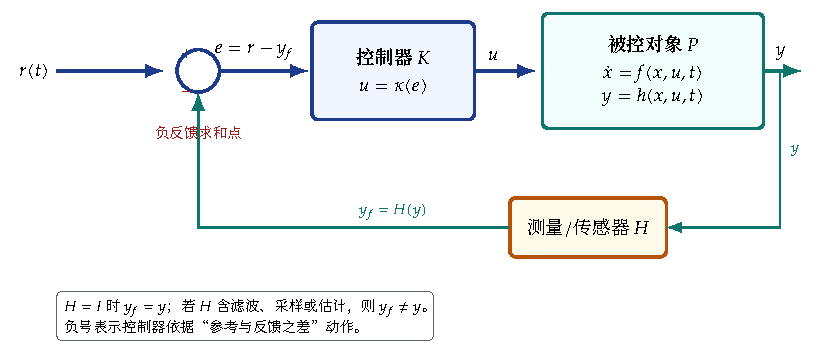
\includegraphics[width=0.94\textwidth]{figures/fig4-feedback.pdf}
\caption{闭环负反馈框图。读图要点：$r$ 是参考输入，$y_f=H(y)$ 是反馈量，求和点处的负号给出 $e=r-y_f$；控制器 $K$ 根据 $e$ 产生 $u$，被控对象 $P$ 产生 $y$。若 $H=I$，则 $y_f=y$；若 $H$ 含滤波、采样或状态估计，则 $y_f\ne y$，设计中必须把 $H$ 的动态一并考虑。}
\label{fig:feedback}
\end{figure}

\subsection{从分析到设计：给定 \texorpdfstring{$V$}{V}，选 \texorpdfstring{$u$}{u} 使 \texorpdfstring{$\dot V<0$}{dV/dt<0}}

考虑控制仿射系统
\begin{equation}
  \dot x=f(x)+g(x)u,\qquad f(0)=0,
  \label{eq:control-affine}
\end{equation}
其中 $x\in\R^n$、$u\in\R^m$、$g(x)\in\R^{n\times m}$。设 $V$ 连续可微、正定。沿 \eqref{eq:control-affine}，
\begin{equation}
  \dot V(x,u)=\nabla V(x)^\top f(x)+\nabla V(x)^\top g(x)u
  =\Lf V(x)+\Lg V(x)u,
  \label{eq:lie-derivative}
\end{equation}
其中 $\Lf V=\nabla V^\top f$ 是标量，$\Lg V=\nabla V^\top g$ 是 $1\times m$ 的行向量。这两个符号称为李导数。

如果 $\Lg V(x)\ne0$，那么 $u$ 可以直接“压”住 $\Lf V$。给定期望的耗散率 $W(x)>0$，取
\begin{equation}
  u(x)=-\frac{(\Lg V(x))^\top}{\norm{\Lg V(x)}^2}\left(\Lf V(x)+W(x)\right),
  \label{eq:one-step}
\end{equation}
则
\begin{equation}
  \dot V=\Lf V-\left(\Lf V+W\right)=-W<0.
\end{equation}
这就是最直接的“给定 $V$、选 $u$”公式。它要求 $\Lg V\ne0$，即 $V$ 必须对输入方向敏感；如果 $\Lg V=0$，则输入无法瞬时影响 $V$，只能依靠 $\Lf V<0$ 自然下降，或者先通过积分/动态扩展把输入“传”到 $V$ 上。

\subsection{控制李雅普诺夫函数（CLF）的基本流程}

\begin{definition}[控制李雅普诺夫函数]
对系统 \eqref{eq:control-affine}，连续可微、正定、径向无界的函数 $V:\R^n\to\R$ 称为控制李雅普诺夫函数（CLF），如果存在连续正定函数 $W$，使得对每个 $x\ne0$，都存在 $u\in\R^m$ 满足
\begin{equation}
  \Lf V(x)+\Lg V(x)u\le -W(x)<0.
  \label{eq:clf}
\end{equation}
\end{definition}

CLF 把“稳定性”翻译成一个逐点的可行性问题：在每个状态 $x$，找一个控制 $u$ 使 $V$ 下降。它的基本流程可以写成五步：
\begin{enumerate}[label=\textbf{步骤 \arabic*}：]
  \item \textbf{建模。}把系统写成 \eqref{eq:control-affine}，确认 $f(0)=0$、$g$ 的列满秩或至少可控方向正确。
  \item \textbf{选 $V$。}优先用物理能量、二次型 $x^\top Px$、线性化后的 Lyapunov 方程解，或“能量 + 误差惩罚”的组合。
  \item \textbf{算李导数。}计算 $\Lf V$ 与 $\Lg V$，检查在 $x\ne0$ 时是否至少有一个方向可使 $\dot V<0$。
  \item \textbf{选控制。}若 $\Lg V\ne0$，可用 \eqref{eq:one-step}；若希望控制幅值最小，用逐点最小范数解
  \begin{equation}
    u_{\mathrm{pm}}(x)=
    \begin{cases}
      0, & \Lf V(x)+W(x)\le0,\\[3pt]
      -\dfrac{(\Lf V+W)(\Lg V)^\top}{\norm{\Lg V}^2}, & \Lf V(x)+W(x)>0,
    \end{cases}
    \label{eq:min-norm}
  \end{equation}
  它在满足 $\dot V\le-W$ 的所有 $u$ 中使 $\norm{u}$ 最小。
  \item \textbf{验证与仿真。}确认 $\dot V\le-W$、检查控制饱和、估计吸引域、做数值仿真；若 $V$ 只给出半负定，改用 LaSalle 或 Barbalat。
\end{enumerate}

CLF 的存在性与可镇定性之间有深刻联系。Artstein 证明，在控制仿射系统的适当正则性条件下，存在 CLF 与系统可渐近镇定是等价的（允许松弛控制）\cite{Artstein1983}；Sontag 进一步给出了一个显式的“万能”控制公式\cite{Sontag1989}。这两条结果把“找 CLF”从一个纯技巧提升为有理论保证的设计框架。

\subsection{Sontag 公式}

设 $V$ 是一个 CLF。记
\begin{equation}
  a(x)=\Lf V(x),\qquad b(x)=\norm{\Lg V(x)}^2=\Lg V(x)(\Lg V(x))^\top\ge0.
\end{equation}
Sontag 的万能公式是
\begin{equation}
  u(x)=
  \begin{cases}
    -\dfrac{a(x)+\sqrt{a(x)^2+b(x)^2}}{b(x)}\,(\Lg V(x))^\top, & b(x)>0,\\[8pt]
    0, & b(x)=0.
  \end{cases}
  \label{eq:sontag}
\end{equation}
当 $b>0$ 时，直接计算：
\begin{equation}
  \dot V=a+\Lg V\,u
  =a-\left(a+\sqrt{a^2+b^2}\right)
  =-\sqrt{a^2+b^2}<0.
\end{equation}
当 $b=0$ 时，CLF 条件 \eqref{eq:clf} 迫使 $a<0$（否则不存在任何 $u$ 能使 $\dot V<0$），所以 $u=0$ 仍然使 $\dot V=a<0$。因此 \eqref{eq:sontag} 对任意 CLF 都有效，且在每个 $x\ne0$ 处严格下降；在原点令 $u(0)=0$ 即可。

\begin{keybox}[Sontag 公式的读法]
分子 $a+\sqrt{a^2+b^2}$ 永远为正（即使 $a$ 很负，根号也把它拉回正），因此控制方向由 $-(\Lg V)^\top$ 决定；分母 $b=\norm{\Lg V}^2$ 起归一化作用。公式的优点是“对任何 CLF 都能用、不需要逐点解优化”，缺点是当 $\norm{\Lg V}$ 很小时控制量可能很大，且它不保证控制最优。工程上常把 $\sqrt{a^2+b^2}$ 换成带饱和/阻尼的修正项，以降低控制幅值。
\end{keybox}

\subsection{LQR 与 HJB 在设计中的位置}

LQR 可以看作“二次型 CLF + 最优增益”的特例：$V=x^\top Px$，$u=-R^{-1}B^\top Px$，其中 $P$ 由 ARE \eqref{eq:are} 给出。对非线性系统，可以在平衡点线性化，先用 LQR 得到一个局部 CLF，再把非线性项作为修正；更系统的做法是求解 HJB 方程，或采用状态依赖 Riccati 方程（SDRE）在每个工作点重解 ARE。CLF 方法与 LQR 的差别在于：LQR 追求二次代价最优，CLF 只要求稳定；因此 CLF 的可行集更大，但控制可能更保守或更“急”。

\subsection{反步法：把 \texorpdfstring{$V$}{V} 一层层“加”出来}

反步法（backstepping）适用于严格反馈形式
\begin{align}
  \dot x_1&=f_1(x_1)+g_1(x_1)x_2,\notag\\
  \dot x_2&=f_2(x_1,x_2)+g_2(x_1,x_2)x_3,\notag\\
  &\ \vdots\notag\\
  \dot x_n&=f_n(x_1,\dots,x_n)+g_n(x_1,\dots,x_n)u.
  \label{eq:strict-feedback}
\end{align}
它的思想是：把 $x_2$ 当作稳定 $x_1$ 的“虚拟控制”，设计一个期望值 $\alpha_1(x_1)$；然后令 $z_2=x_2-\alpha_1(x_1)$，把 $z_2$ 作为新的误差状态，再把 $x_3$ 当作稳定 $z_2$ 的虚拟控制；如此逐层递推，最后得到实际的 $u$。每一步都把上一步的 Lyapunov 函数加上新的误差平方项，因此 $V$ 是“构造出来”的，而不是猜出来的。

用最简单的二阶积分链说明：
\begin{equation}
  \dot x_1=x_2,\qquad \dot x_2=u.
\end{equation}
第一步，取 $V_1=\frac12x_1^2$，希望 $\dot x_1=x_2$ 使 $V_1$ 下降，于是取虚拟控制 $\alpha_1(x_1)=-k_1x_1$（$k_1>0$）。定义误差
\begin{equation}
  z_2=x_2-\alpha_1(x_1)=x_2+k_1x_1.
\end{equation}
第二步，取
\begin{equation}
  V_2=V_1+\frac12z_2^2=\frac12x_1^2+\frac12(x_2+k_1x_1)^2.
\end{equation}
沿轨迹
\begin{align}
  \dot V_2
  &=x_1x_2+z_2(\dot x_2+k_1\dot x_1)\notag\\
  &=x_1x_2+z_2(u+k_1x_2)\notag\\
  &=-k_1x_1^2+z_2\left(x_1+u+k_1x_2\right).
\end{align}
取
\begin{equation}
  u=-x_1-k_1x_2-k_2z_2,\qquad k_2>0,
\end{equation}
则
\begin{equation}
  \dot V_2=-k_1x_1^2-k_2z_2^2<0.
\end{equation}
$V_2$ 正定且径向无界，于是闭环全局渐近稳定。这个例子是线性的，但递推结构对非线性 $f_i,g_i$ 同样适用；关键是每一步都能把交叉项“配”成负平方。

\begin{warnbox}[反步法的适用范围]
反步法要求系统具有三角形（严格反馈）结构，且每一步的 $g_i$ 不为零、函数足够光滑。对非三角形系统、输入受约束系统或高维系统，反步法会产生“复杂度爆炸”（对虚拟控制反复求导导致项数急剧增长），工程上常结合动态面控制、命令滤波或神经网络近似来缓解。
\end{warnbox}

\subsection{滑模控制：把 \texorpdfstring{$V$}{V} 用在“到达”阶段}

滑模控制（sliding mode control）先设计一个滑动变量 $s(x)$，使 $s=0$ 的滑动面上有良好的降阶动力学；再设计 $u$ 迫使 $s$ 在有限时间内到达 $0$。到达阶段常用
\begin{equation}
  V(s)=\frac12s^2
\end{equation}
作为 Lyapunov 函数，要求
\begin{equation}
  \dot V=s\dot s\le-\eta\abs{s},\qquad \eta>0.
  \label{eq:reaching}
\end{equation}
这保证 $\abs{s}$ 以至少 $\eta$ 的速率下降，从而在有限时间到达 $s=0$。例如对 $\dot x=f(x)+g(x)u$（标量），取 $s=x$，控制
\begin{equation}
  u=-\frac{1}{g(x)}\left(f(x)+k\,\operatorname{sign}(s)\right),\qquad k>0,
\end{equation}
则 $s\dot s=-k\abs{s}$，满足 \eqref{eq:reaching}。到达之后，系统被“约束”在 $s=0$ 上，只需分析降阶后的滑动模态稳定性。

需要强调：$V=\frac12s^2$ 只是\textbf{到达阶段}的 Lyapunov 函数，它并不自动保证整个状态收敛到原点；滑动面上的稳定性要单独设计。此外，符号函数 $\operatorname{sign}(s)$ 在 $s=0$ 附近的高频切换会引起抖振（chattering），工程上用饱和函数、边界层或高阶滑模来抑制。

\subsection{自适应控制：把参数误差也放进 \texorpdfstring{$V$}{V}}

自适应控制处理“模型有未知常数参数”的情形。设
\begin{equation}
  \dot x=\theta x+u,
\end{equation}
其中 $\theta$ 是未知常数，$x,u\in\R$。取估计 $\hat\theta$，控制
\begin{equation}
  u=-\hat\theta x-kx,\qquad k>0.
\end{equation}
定义参数误差 $\tilde\theta=\theta-\hat\theta$，候选 Lyapunov 函数
\begin{equation}
  V(x,\tilde\theta)=\frac12x^2+\frac{1}{2\gamma}\tilde\theta^2,\qquad \gamma>0.
\end{equation}
沿闭环
\begin{align}
  \dot V
  &=x(\theta x+u)-\frac{1}{\gamma}\tilde\theta\dot{\hat\theta}\notag\\
  &=x(\tilde\theta x-kx)-\frac{1}{\gamma}\tilde\theta\dot{\hat\theta}\notag\\
  &=-kx^2+\tilde\theta\left(x^2-\frac{1}{\gamma}\dot{\hat\theta}\right).
\end{align}
选择自适应律
\begin{equation}
  \dot{\hat\theta}=\gamma x^2,
  \label{eq:adaptation}
\end{equation}
则交叉项被抵消，
\begin{equation}
  \dot V=-kx^2\le0.
\end{equation}
由 LaSalle（或 Barbalat）可证 $x(t)\to0$。但要注意：$\dot V=-kx^2$ 只是半负定，不满足定理~\ref{thm:global} 的负定条件；用 LaSalle 时，$E=\{x=0\}$ 中包含任意常数参数误差，最大不变集不是 $\{0\}$，因此只能断言状态收敛，不能断言 $\tilde\theta\to0$。参数误差通常还需要持续激励（persistency of excitation）才能收敛到零。实际中还会加入投影、$\sigma$-修正或死区，以防止参数漂移和噪声放大。

\subsection{设计方法对照}

表~\ref{tab:methods} 把本节讨论的方法放在同一张表里。它们的共同点是：都围绕一个标量 $V$ 做文章；区别在于 $V$ 怎么选、$u$ 怎么定、以及保证的是渐近稳定、有限时间还是参数收敛。

\begin{table}[H]
\centering
\small
\begin{tabularx}{\textwidth}{@{}>{\raggedright\arraybackslash}p{2.1cm}>{\raggedright\arraybackslash}p{3.0cm}>{\raggedright\arraybackslash}p{3.4cm}>{\raggedright\arraybackslash}p{3.1cm}X@{}}
\toprule
方法 & 典型 $V$ & 控制律/设计 & 保证 & 主要局限 \\
\midrule
CLF 逐点最小范数 & 二次型、能量型 & 解 $\dot V\le-W$，取 $\norm{u}$ 最小 & 渐近稳定，控制幅值较小 & 需 CLF；$\Lg V=0$ 处可能不连续 \\
Sontag 公式 & 任意 CLF & 显式公式 \eqref{eq:sontag} & 对任意 CLF 严格下降 & 控制可能很大；非最优 \\
LQR & $x^\top Px$ & 解 ARE，$u=-Kx$ & 线性系统全局指数稳定、二次最优 & 仅线性/局部线性化；需 $R>0$ \\
反步法 & 逐层构造的 $V$ & 虚拟控制 + 递推 & 严格反馈系统全局稳定 & 需三角形结构；复杂度爆炸 \\
滑模 & $\frac12s^2$（到达阶段） & 到达条件 $s\dot s\le-\eta\abs{s}$ & 有限时间到达；滑动面稳定 & 抖振；需切换增益 \\
自适应 & 状态 + 参数误差 & 自适应律抵消交叉项 & 状态收敛；参数需持续激励 & 参数漂移；未建模动态 \\
\bottomrule
\end{tabularx}
\caption{常见 Lyapunov 设计方法对照。所有方法都以一个标量 $V$ 为核心，但 $V$ 的构造与控制律的来源不同。}
\label{tab:methods}
\end{table}

% ============================================================================
\section{闭环设计例子：从 \texorpdfstring{$V$}{V} 到 \texorpdfstring{$u$}{u} 的完整流程}
\label{sec:example}
% ============================================================================

\subsection{被控对象与开环问题}

考虑二阶非线性系统
\begin{equation}
  \dot x_1=-x_1^3+x_2,\qquad \dot x_2=u,\qquad y=x_1,
  \label{eq:example-plant}
\end{equation}
其中 $x=(x_1,x_2)^\top\in\R^2$，$u\in\R$，$y\in\R$。写成控制仿射形式：
\begin{equation}
  f(x)=\begin{pmatrix}-x_1^3+x_2\\0\end{pmatrix},\qquad
  g(x)=\begin{pmatrix}0\\1\end{pmatrix}.
\end{equation}
开环（$u=0$）时，$\dot x_2=0$，故 $x_2\equiv x_2(0)$ 为常数；$\dot x_1=-x_1^3+x_2$ 的平衡点满足 $x_1^3=x_2$。因此开环系统有一整条平衡点集 $\{(x_1,x_2):x_2=x_1^3\}$，原点只是其中一点，且并不吸引：若 $x_2(0)\ne0$，$x_1(t)$ 会收敛到 $x_2(0)^{1/3}$ 而不是 $0$。所以必须设计反馈。

\subsection{选取 \texorpdfstring{$V$}{V} 并设计 \texorpdfstring{$u$}{u}}

取最简单的二次型
\begin{equation}
  V(x)=\frac12\left(x_1^2+x_2^2\right).
\end{equation}
它正定、径向无界。计算李导数：
\begin{align}
  \Lf V&=\nabla V^\top f
  =x_1(-x_1^3+x_2)+x_2\cdot0=-x_1^4+x_1x_2,\\
  \Lg V&=\nabla V^\top g
  =\begin{pmatrix}x_1&x_2\end{pmatrix}\begin{pmatrix}0\\1\end{pmatrix}=x_2.
\end{align}
于是
\begin{equation}
  \dot V=-x_1^4+x_1x_2+x_2u.
\end{equation}
选择
\begin{equation}
  u=-x_1-kx_2,\qquad k>0,
  \label{eq:example-control}
\end{equation}
则交叉项 $x_1x_2$ 被抵消：
\begin{equation}
  \dot V=-x_1^4+x_1x_2+x_2(-x_1-kx_2)
  =-x_1^4-kx_2^2<0,\qquad x\ne0.
  \label{eq:example-dotV}
\end{equation}
这是一个简单而完整的 CLF 设计：$V$ 给定，$u$ 的选择直接来自“让 $\dot V$ 负定”的要求。值得注意的是，控制律 \eqref{eq:example-control} 并不需要取消非线性项 $-x_1^3$；非线性项本身已经在帮助耗散能量（$-x_1^4$），控制只需处理交叉项与提供阻尼。

\subsection{稳定性证明}

\begin{proposition}
对任意 $k>0$，闭环系统 \eqref{eq:example-plant}--\eqref{eq:example-control} 的原点是全局渐近稳定的。
\end{proposition}

\begin{proof}
闭环为
\begin{equation}
  \dot x_1=-x_1^3+x_2,\qquad \dot x_2=-x_1-kx_2.
  \label{eq:example-closed}
\end{equation}
右端是多项式，局部 Lipschitz。取 $V=\frac12(x_1^2+x_2^2)$，它正定、连续可微且径向无界。由 \eqref{eq:example-dotV}，
\begin{equation}
  \dot V=-x_1^4-kx_2^2<0,\qquad \forall\,x\ne0.
\end{equation}
令 $W(x)=x_1^4+kx_2^2$，它连续正定。因此定理~\ref{thm:global} 的全部条件满足，原点是全局渐近稳定的。证毕。
\end{proof}

\begin{remark}[与线性化的关系]
在原点线性化 \eqref{eq:example-closed}：
\begin{equation}
  A=\begin{pmatrix}0&1\\-1&-k\end{pmatrix}.
\end{equation}
特征多项式为 $\lambda^2+k\lambda+1=0$。对 $k>0$，两个特征值的实部都是 $-k/2<0$，故原点局部指数稳定。但线性化只能给出局部结论；上面的 $V$ 给出了全局结论，而且给出了显式的“能量”证书。
\end{remark}

\subsection{仿真与讨论}

取 $k=2$，对多个初值做数值仿真。图~\ref{fig:example-sim} 左图是闭环相图，右图是初值 $(2,1)$ 的时间响应。所有轨迹都收敛到原点；$x_1,x_2$ 单调或略带振荡地衰减，控制 $u$ 在初始阶段较大（$u(0)=-2-2\cdot1=-4$），随后趋于零。

\begin{figure}[H]
\centering
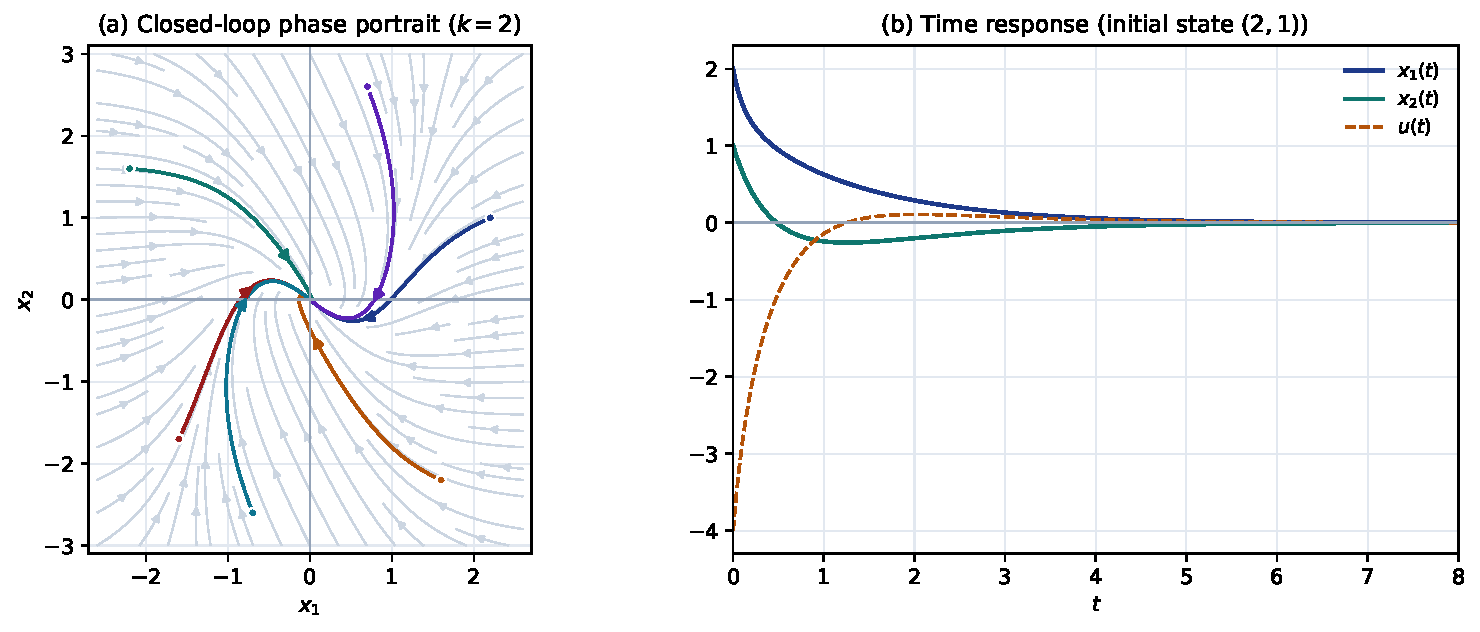
\includegraphics[width=\textwidth]{figures/fig5-closed-loop.pdf}
\caption{闭环系统 \eqref{eq:example-closed} 的仿真（$k=2$）。读图要点：左图相平面中，不同初值的轨迹都指向原点，说明原点吸引；灰色箭头是向量场方向，彩色曲线是若干条数值轨迹。右图给出初值 $(2,1)$ 的 $x_1(t)$、$x_2(t)$ 与 $u(t)$：状态收敛到零，控制最终归零；初始控制幅值约为 $4$，若执行器饱和小于该值，则需要重新设计或加入抗饱和措施。}
\label{fig:example-sim}
\end{figure}

这个例子还揭示了两个实践要点。第一，\textbf{$V$ 不必很复杂}：二次型已经足够，因为非线性项 $-x_1^3$ 本身提供了 $-x_1^4$ 的耗散；如果被控对象有更复杂的非线性，可以先用线性化/LQR 得到一个二次型 $V$，再根据 $\dot V$ 的符号补上非线性修正项。第二，\textbf{控制律不是唯一的}：满足 $\dot V<0$ 的 $u$ 有很多，式 \eqref{eq:example-control} 只是其中一个简单的选择；若用逐点最小范数 \eqref{eq:min-norm} 或 Sontag 公式 \eqref{eq:sontag}，会得到不同的控制律，但稳定性保证相同。工程上应根据控制幅值、执行器带宽和鲁棒性在可行控制律中挑选。

\begin{warnbox}[输入饱和的提醒]
本例中 $u=-x_1-kx_2$ 是线性的，但初始状态较大时控制幅值也大。如果真实执行器满足 $\abs{u}\le u_{\max}$，那么在大误差阶段实际施加的是饱和控制，$\dot V<0$ 的推导不再成立。此时需要：减小初始吸引域、使用饱和感知的 CLF、加入抗饱和补偿，或改用模型预测控制（MPC）。Lyapunov 分析给出的是“理想控制”下的保证，不能替代对执行器约束的检查。
\end{warnbox}

% ============================================================================
\section{适用范围、局限与总结}
\label{sec:scope}
% ============================================================================

\subsection{适用范围}

Lyapunov 方法适用于相当广泛的一类系统：线性与非线性、连续与离散、自治与非自治、有限维与无穷维（后者需要把 $V$ 换成 Lyapunov 泛函）。本文给出的三个定理针对连续时间自治系统；对非自治系统，需要把“稳定”加强为一致稳定，把 $V$ 换成含时间的 $V(x,t)$，并使用 $\mathcal{K}$、$\mathcal{KL}$ 类函数与 Barbalat 引理。对离散系统，把 $\dot V$ 换成差分 $\Delta V=V(x_{k+1})-V(x_k)$ 即可，结论形式完全类似。对带扰动的系统，输入-状态稳定性（ISS）把“无扰动时收敛”推广为“扰动有界时状态有界”，其 Lyapunov 版本是 ISS-Lyapunov 函数\cite{SontagWang1995}。

\subsection{局限}

\begin{enumerate}[label=(\arabic*)]
  \item \textbf{充分性而非必要性。}找到一个 $V$ 证明稳定；找不到 $V$ 不能证明不稳定。逆定理虽然保证渐近稳定系统存在 Lyapunov 函数，但通常是非构造性的。
  \item \textbf{构造 $V$ 没有万能算法。}对低维系统可以猜能量、猜二次型；对高维系统，常用平方和（SOS）优化、线性矩阵不等式（LMI）、神经网络 Lyapunov 函数等方法，但都有计算复杂度或保守性\cite{Boyd1994}。
  \item \textbf{条件偏保守。}$\dot V$ 负定是充分条件，很多系统只需要 LaSalle 的半负定条件；反过来，若 $V$ 选得不好，即使系统稳定也可能验证失败。
  \item \textbf{对模型误差与扰动敏感。}Lyapunov 函数是针对名义模型构造的；未建模动态、参数漂移、噪声与饱和可能破坏 $\dot V<0$。鲁棒 Lyapunov 函数、ISS、自适应与滑模都是为应对这一点而发展的。
  \item \textbf{非自治系统的额外困难。}LaSalle 不变集原理不能直接用于非自治系统；一致渐近稳定需要 $V(x,t)$ 具有递减的 $\mathcal{K}$ 界，证明通常更繁琐。
  \item \textbf{控制幅值与可行性。}CLF 只保证“存在 $u$”，不保证 $\abs{u}$ 在执行器范围内；Sontag 公式在 $\norm{\Lg V}$ 很小时可能给出很大的控制。实际设计必须把饱和、带宽与采样率纳入。
\end{enumerate}

\subsection{实践检查清单}

把 Lyapunov 方法用于一个具体问题时，可以按下面的顺序检查：
\begin{enumerate}[label=\textbf{\arabic*.}]
  \item 把平衡点平移到原点，写出状态方程，确认 $f(0)=0$ 或闭环平衡点；
  \item 判断是自治还是非自治、局部还是全局、连续还是离散；
  \item 选一个候选 $V$：优先物理能量、二次型、线性化 Lyapunov 方程解、或“能量 + 误差”组合；
  \item 计算 $\dot V$，先看符号，再看是否负定；若只是半负定，尝试 LaSalle；
  \item 检查 $V$ 是否正定、径向无界；若只局部，估计子水平集 $\Omega_c$；
  \item 根据定理~\ref{thm:stable}、\ref{thm:asym}、\ref{thm:global} 或 LaSalle 下结论；
  \item 检查控制幅值、饱和、噪声与未建模动态，做数值仿真验证；
  \item 若验证失败，换 $V$、换坐标、加积分/自适应/鲁棒项，或缩小吸引域。
\end{enumerate}

\subsection{总结}

李雅普诺夫方法把“稳定性”从一个关于解的渐近行为的问题，转化成一个关于标量函数 $V$ 及其沿轨迹导数 $\dot V$ 的符号问题。三个定理构成一条清晰的层次链：
\begin{itemize}
  \item $V$ 正定、$\dot V\le0$ $\Rightarrow$ 稳定（定理~\ref{thm:stable}）；
  \item 再加 $\dot V$ 负定 $\Rightarrow$ 渐近稳定（定理~\ref{thm:asym}）；
  \item 再加 $V$ 径向无界 $\Rightarrow$ 全局渐近稳定（定理~\ref{thm:global}）。
\end{itemize}
证明的核心始终是“用 $V$ 的等值面当围栏”：定理~\ref{thm:stable} 用球面上的最小值 $m$ 阻止轨迹穿出；定理~\ref{thm:asym} 用 $V$ 的极限与紧环上的正下界把轨迹逼回原点；定理~\ref{thm:global} 用径向无界把每个子水平集变成紧集，从而把局部论证推广到全空间。LaSalle 不变集原理则在 $\dot V$ 半负定时提供了更强的收敛判据。

在控制设计中，Lyapunov 方法从“分析工具”变成“设计工具”：给定 $V$，把 $\dot V<0$ 当作对 $u$ 的约束，就得到 CLF；选择不同的约束（最小范数、Sontag 公式、LQR 最优、反步递推、滑模到达、自适应律）就得到不同的控制律。线性系统的 Lyapunov 方程与 LQR 的 ARE 是这一框架最成熟的特例；非线性系统的 CLF、反步、滑模与自适应则是它在不同结构下的展开。真正困难的从来不是“验证一个给定的 $V$”，而是“为一个具体系统构造一个既不过分保守、又能指导控制的 $V$”；这既是理论问题，也是工程艺术。

% ============================================================================
\begin{thebibliography}{99}
% ============================================================================

\bibitem{Lyapunov1892}
A. M. Lyapunov.
\newblock \emph{The General Problem of the Stability of Motion}.
\newblock Translated by A. T. Fuller. Taylor \& Francis, London, 1992.
\newblock (Original Russian edition: Kharkov, 1892.)

\bibitem{LaSalle1960}
J. P. LaSalle.
\newblock Some extensions of Liapunov's second method.
\newblock \emph{IRE Transactions on Circuit Theory}, 7(4):520--527, 1960.
\newblock \href{https://doi.org/10.1109/TCT.1960.1086720}{doi:10.1109/TCT.1960.1086720}.

\bibitem{Massera1949}
J. L. Massera.
\newblock On Liapounoff's conditions of stability.
\newblock \emph{Annals of Mathematics}, 50(3):705--721, 1949.
\newblock \href{https://doi.org/10.2307/1969558}{doi:10.2307/1969558}.

\bibitem{Hahn1967}
W. Hahn.
\newblock \emph{Stability of Motion}.
\newblock Springer-Verlag, Berlin, 1967.

\bibitem{Khalil2002}
H. K. Khalil.
\newblock \emph{Nonlinear Systems}, 3rd edition.
\newblock Prentice Hall, Upper Saddle River, NJ, 2002.

\bibitem{Artstein1983}
Z. Artstein.
\newblock Stabilization with relaxed controls.
\newblock \emph{Nonlinear Analysis: Theory, Methods \& Applications}, 7(11):1163--1173, 1983.
\newblock \href{https://doi.org/10.1016/0362-546X(83)90049-4}{doi:10.1016/0362-546X(83)90049-4}.

\bibitem{Sontag1989}
E. D. Sontag.
\newblock A ``universal'' construction of Artstein's theorem on nonlinear stabilization.
\newblock \emph{Systems \& Control Letters}, 13(2):117--123, 1989.
\newblock \href{https://doi.org/10.1016/0167-6911(89)90028-5}{doi:10.1016/0167-6911(89)90028-5}.

\bibitem{Sontag1990}
E. D. Sontag.
\newblock \emph{Mathematical Control Theory: Deterministic Finite Dimensional Systems}.
\newblock Springer-Verlag, New York, 1990.

\bibitem{Sepulchre1997}
R. Sepulchre, M. Jankovi\'c, and P. V. Kokotovi\'c.
\newblock \emph{Constructive Nonlinear Control}.
\newblock Springer-Verlag, London, 1997.

\bibitem{Krstic1995}
M. Krsti\'c, I. Kanellakopoulos, and P. V. Kokotovi\'c.
\newblock \emph{Nonlinear and Adaptive Control Design}.
\newblock John Wiley \& Sons, New York, 1995.

\bibitem{Slotine1991}
J.-J. E. Slotine and W. Li.
\newblock \emph{Applied Nonlinear Control}.
\newblock Prentice Hall, Englewood Cliffs, NJ, 1991.

\bibitem{Anderson2007}
B. D. O. Anderson and J. B. Moore.
\newblock \emph{Optimal Control: Linear Quadratic Methods}.
\newblock Dover Publications, Mineola, NY, 2007.

\bibitem{Boyd1994}
S. Boyd, L. El Ghaoui, E. Feron, and V. Balakrishnan.
\newblock \emph{Linear Matrix Inequalities in System and Control Theory}.
\newblock SIAM, Philadelphia, 1994.

\bibitem{SontagWang1995}
E. D. Sontag and Y. Wang.
\newblock On characterizations of the input-to-state stability property.
\newblock \emph{Systems \& Control Letters}, 24(5):351--359, 1995.
\newblock \href{https://doi.org/10.1016/0167-6911(94)00050-6}{doi:10.1016/0167-6911(94)00050-6}.

\bibitem{Isidori1995}
A. Isidori.
\newblock \emph{Nonlinear Control Systems}, 3rd edition.
\newblock Springer-Verlag, London, 1995.

\end{thebibliography}

\end{document}
